
\documentclass[a4paper,11pt]{article}

% Package imports
\usepackage{latexsym}
\usepackage[romanian]{babel}
\usepackage{xcolor}
\usepackage{float}
\usepackage{ragged2e}
\usepackage[empty]{fullpage}
\usepackage{wrapfig}
\usepackage{lipsum}
\usepackage{tabularx}
\usepackage{titlesec}
\usepackage{geometry}
\usepackage{marvosym}
\usepackage{verbatim}
\usepackage{enumitem}
\usepackage{fancyhdr}
\usepackage{multicol}
\usepackage{graphicx}
\usepackage{cfr-lm}
\usepackage[T1]{fontenc}
\usepackage{fontawesome5}

\usepackage[absolute]{textpos}
\setlength{\TPHorizModule}{1mm}
\setlength{\TPVertModule}{1mm}

% Color definitions
\definecolor{darkblue}{RGB}{0,0,139}

% Page layout
\setlength{\multicolsep}{0pt} 
\pagestyle{fancy}
\fancyhf{} % clear all header and footer fields
\fancyfoot{}
\renewcommand{\headrulewidth}{0pt}
\renewcommand{\footrulewidth}{0pt}
\geometry{left=1.4cm, top=0.8cm, right=1.2cm, bottom=1cm}
\setlength{\footskip}{5pt} % Addressing fancyhdr warning

% Hyperlink setup (moved after fancyhdr to address warning)
\usepackage[hidelinks]{hyperref}
\hypersetup{
    colorlinks=true,
    linkcolor=darkblue,
    filecolor=darkblue,
    urlcolor=darkblue,
}

% Custom box settings
\usepackage[most]{tcolorbox}
\tcbset{
    frame code={},
    center title,
    left=0pt,
    right=0pt,
    top=0pt,
    bottom=0pt,
    colback=gray!20,
    colframe=white,
    width=\dimexpr\textwidth\relax,
    enlarge left by=-2mm,
    boxsep=4pt,
    arc=0pt,outer arc=0pt,
}

% URL style
\urlstyle{same}

% Text alignment
\raggedright
\setlength{\tabcolsep}{0in}

% Section formatting
\titleformat{\section}{
  \vspace{-4pt}\scshape\raggedright\large
}{}{0em}{}[\color{black}\titlerule \vspace{-7pt}]

% Custom commands
\newcommand{\resumeItem}[2]{
  \item{
    \textbf{#1}{\hspace{0.5mm}#2 \vspace{-0.5mm}}
  }
}

\newcommand{\resumePOR}[3]{
\vspace{0.5mm}\item
    \begin{tabular*}{0.97\textwidth}[t]{l@{\extracolsep{\fill}}r}
        \textbf{#1}\hspace{0.3mm}#2 & \textit{\small{#3}} 
    \end{tabular*}
    \vspace{-2mm}
}

\newcommand{\resumeSubheading}[4]{
\vspace{0.5mm}\item
    \begin{tabular*}{0.98\textwidth}[t]{l@{\extracolsep{\fill}}r}
        \textbf{#1} & \textit{\footnotesize{#4}} \\
        \textit{\footnotesize{#3}} &  \footnotesize{#2}\\
    \end{tabular*}
    \vspace{-2.4mm}
}

\newcommand{\resumeProject}[4]{
\vspace{0.5mm}\item
    \begin{tabular*}{0.98\textwidth}[t]{l@{\extracolsep{\fill}}r}
        \textbf{#1} & \textit{\footnotesize{#3}} \\
        \footnotesize{\textit{#2}} & \footnotesize{#4}
    \end{tabular*}
    \vspace{-2.4mm}
}

% Organisation header with several roles listed under it
\newcommand{\resumeOrg}[2]{
\vspace{0.5mm}\item
    \begin{tabular*}{0.98\textwidth}[t]{l@{\extracolsep{\fill}}r}
        \textbf{#1} & \footnotesize{#2} \\
    \end{tabular*}
    \vspace{-1mm}
}

\newcommand{\resumeRole}[2]{
    \par\vspace{0.3mm}
    \begin{tabular*}{0.98\textwidth}[t]{l@{\extracolsep{\fill}}r}
        \textit{\footnotesize{#1}} & \textit{\footnotesize{#2}} \\
    \end{tabular*}
    \vspace{-2.4mm}
}

\newcommand{\resumeSubItem}[2]{\resumeItem{#1}{#2}\vspace{-4pt}}

\renewcommand{\labelitemi}{$\vcenter{\hbox{\tiny$\bullet$}}$}
\renewcommand{\labelitemii}{$\vcenter{\hbox{\tiny$\circ$}}$}

\newcommand{\resumeSubHeadingListStart}{\begin{itemize}[leftmargin=*,labelsep=1mm]}
\newcommand{\resumeHeadingSkillStart}{\begin{itemize}[leftmargin=*,itemsep=1.7mm, rightmargin=2ex]}
\newcommand{\resumeItemListStart}{\begin{itemize}[leftmargin=*,labelsep=1mm,itemsep=0.5mm]}

\newcommand{\resumeSubHeadingListEnd}{\end{itemize}\vspace{2mm}}
\newcommand{\resumeHeadingSkillEnd}{\end{itemize}\vspace{-2mm}}
\newcommand{\resumeItemListEnd}{\end{itemize}\vspace{-2mm}}
\newcommand{\cvsection}[1]{%
\vspace{2mm}
\begin{tcolorbox}
    \textbf{\large #1}
\end{tcolorbox}
    \vspace{-4mm}
}

\newcolumntype{L}{>{\raggedright\arraybackslash}X}%
\newcolumntype{R}{>{\raggedleft\arraybackslash}X}%
\newcolumntype{C}{>{\centering\arraybackslash}X}%


% Commands for icon sizing and positioning
\newcommand{\socialicon}[1]{\raisebox{-0.05em}{\resizebox{!}{1em}{#1}}}
\newcommand{\ieeeicon}[1]{\raisebox{-0.3em}{\resizebox{!}{1.3em}{#1}}}

% Font options
\newcommand{\headerfonti}{\fontfamily{phv}\selectfont} % Helvetica-like (similar to Arial/Calibri)
\newcommand{\headerfontii}{\fontfamily{ptm}\selectfont} % Times-like (similar to Times New Roman)
\newcommand{\headerfontiii}{\fontfamily{ppl}\selectfont} % Palatino (elegant serif)
\newcommand{\headerfontiv}{\fontfamily{pbk}\selectfont} % Bookman (readable serif)
\newcommand{\headerfontv}{\fontfamily{pag}\selectfont} % Avant Garde-like (similar to Trebuchet MS)
\newcommand{\headerfontvi}{\fontfamily{cmss}\selectfont} % Computer Modern Sans Serif
\newcommand{\headerfontvii}{\fontfamily{qhv}\selectfont} % Quasi-Helvetica (another Arial/Calibri alternative)
\newcommand{\headerfontviii}{\fontfamily{qpl}\selectfont} % Quasi-Palatino (another elegant serif option)
\newcommand{\headerfontix}{\fontfamily{qtm}\selectfont} % Quasi-Times (another Times New Roman alternative)
\newcommand{\headerfontx}{\fontfamily{bch}\selectfont} % Charter (clean serif font)

\begin{document}
\headerfontiii

% Header (kept in a fixed-size box so the page can't squeeze it under the photo)
\noindent\begin{minipage}{\textwidth}
\begin{center}
    {\Huge\textbf{Vlad-Andrei TOMICI}}
\end{center}
\vspace{-6mm}

% \begin{wrapfigure}{l}{0.25\textwidth}
%     \vspace{-20mm}
%     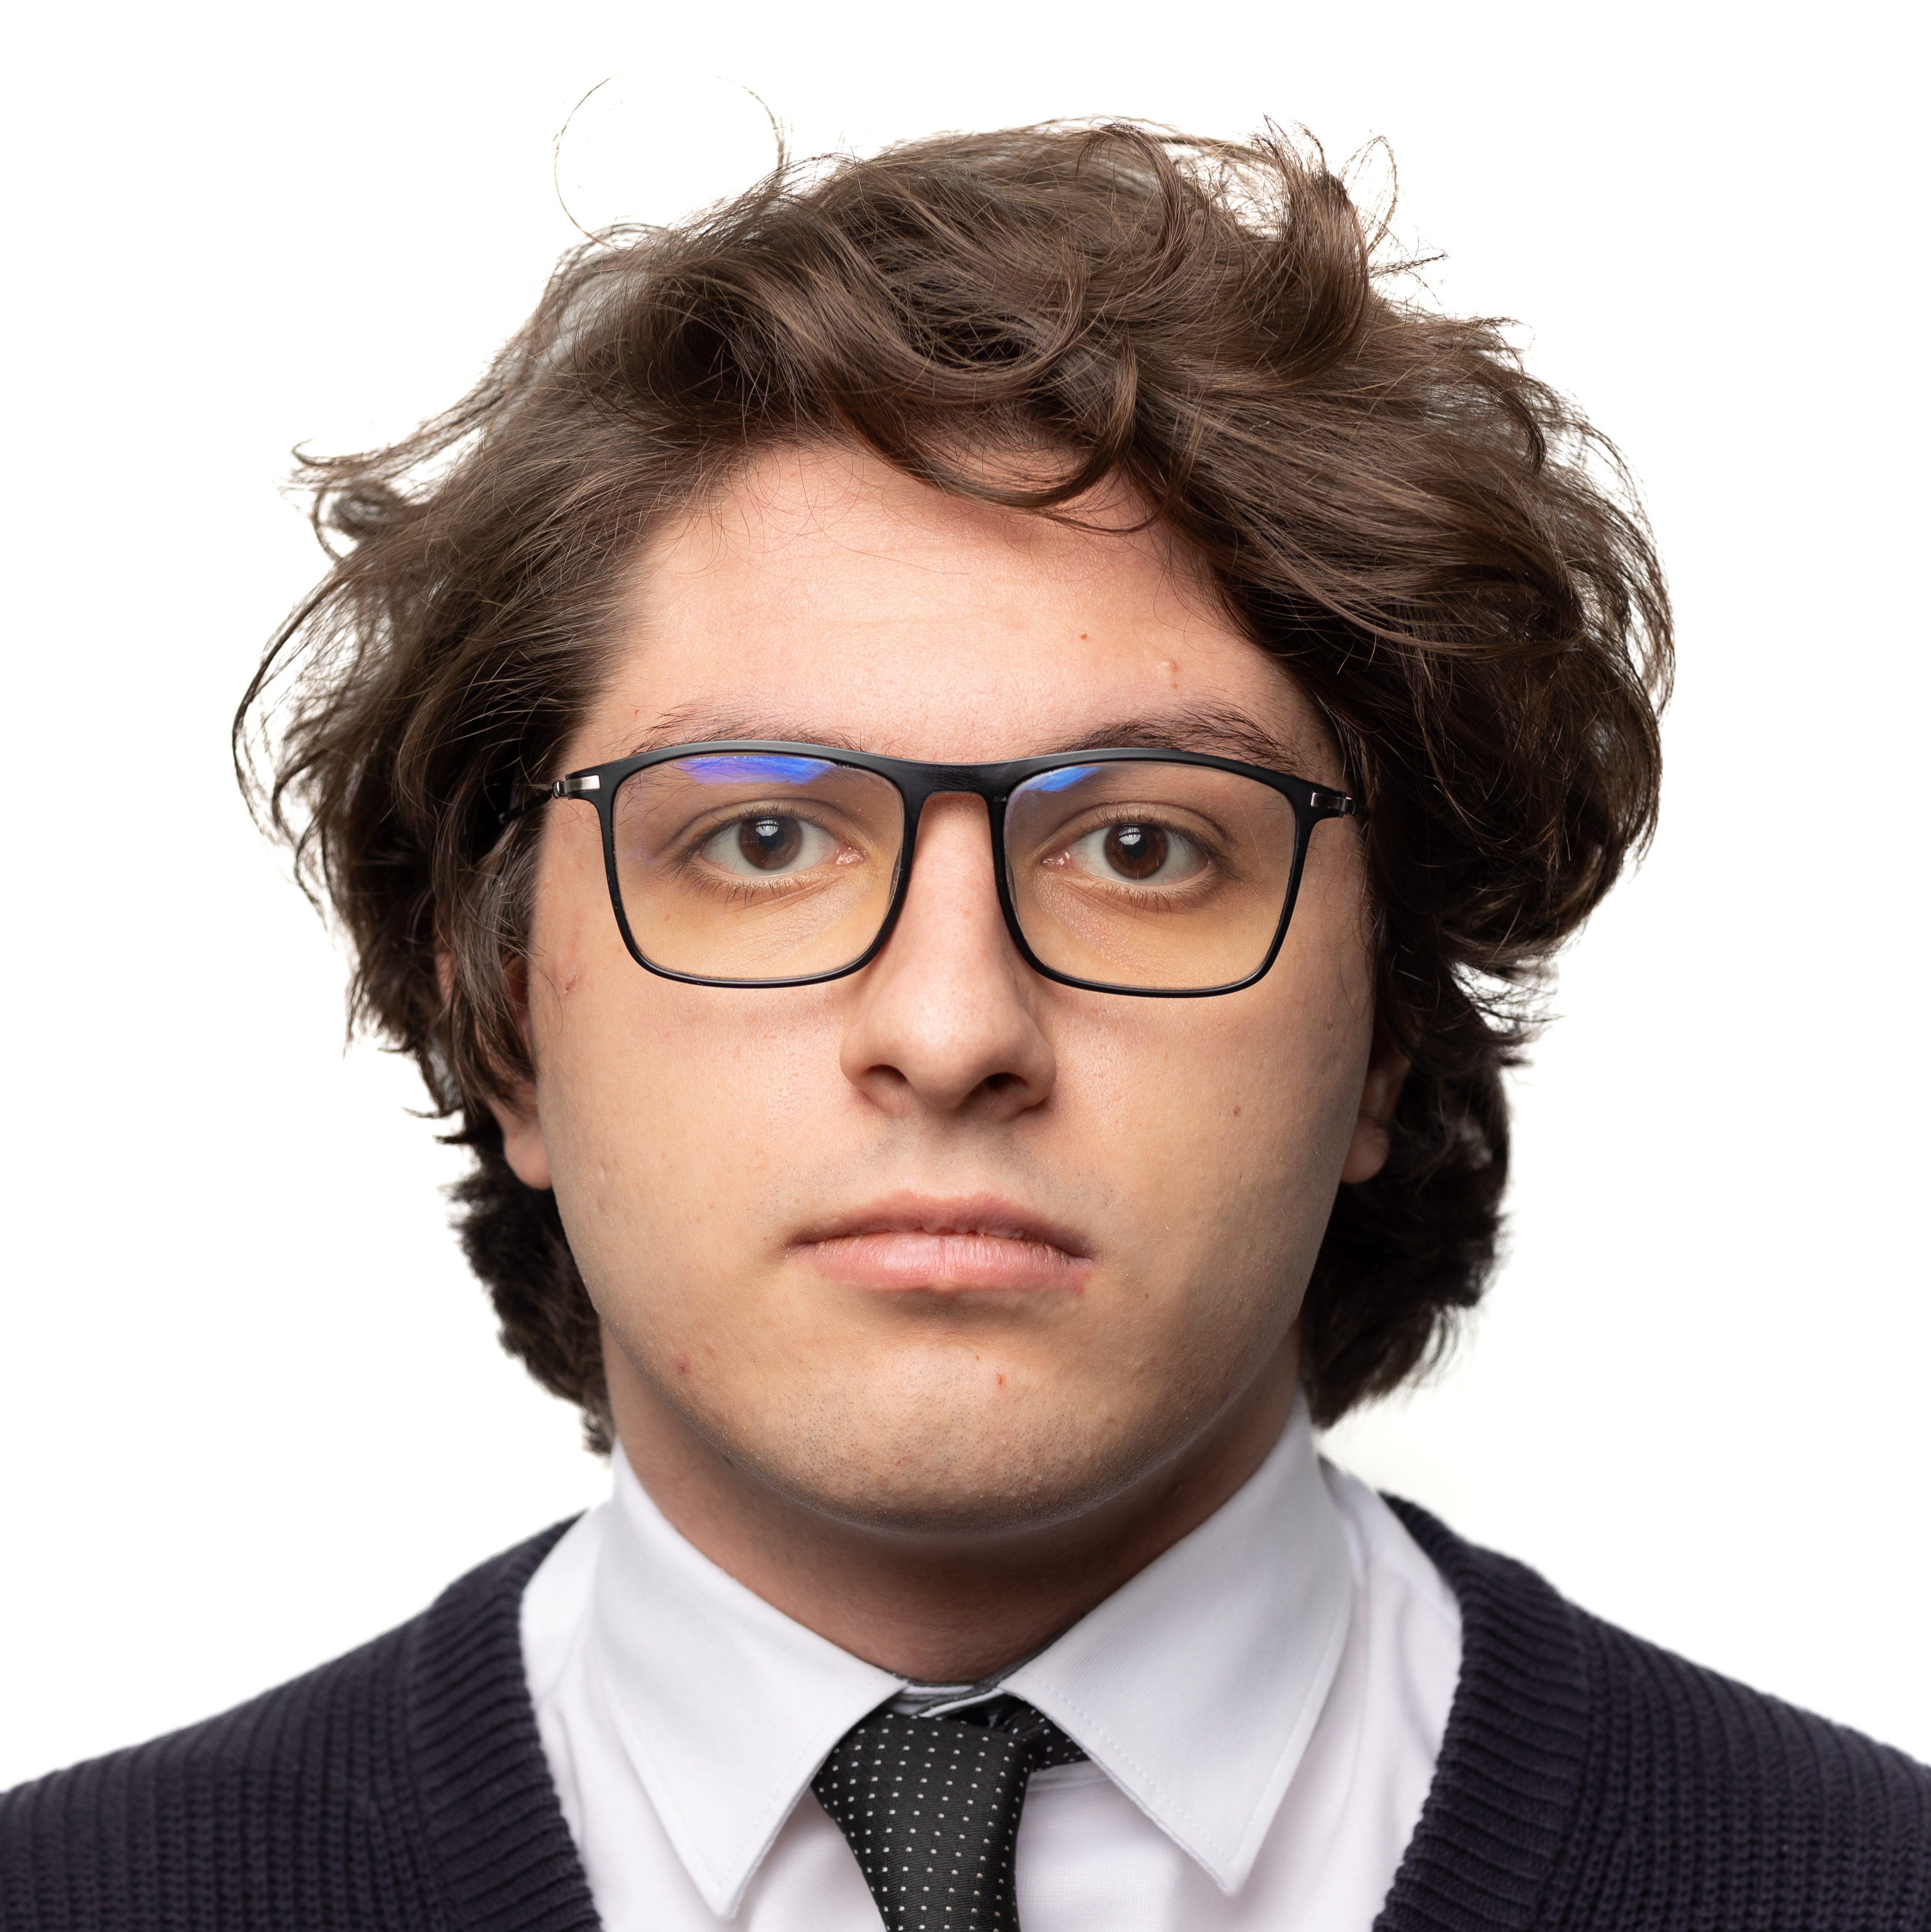
\includegraphics[width=0.25\textwidth]{STOP2008-rect.jpg}
%     \vspace{-10mm}
% \end{wrapfigure}

\begin{textblock}{30}(10, 10) % Adjust the coordinates (10, 10) as needed
    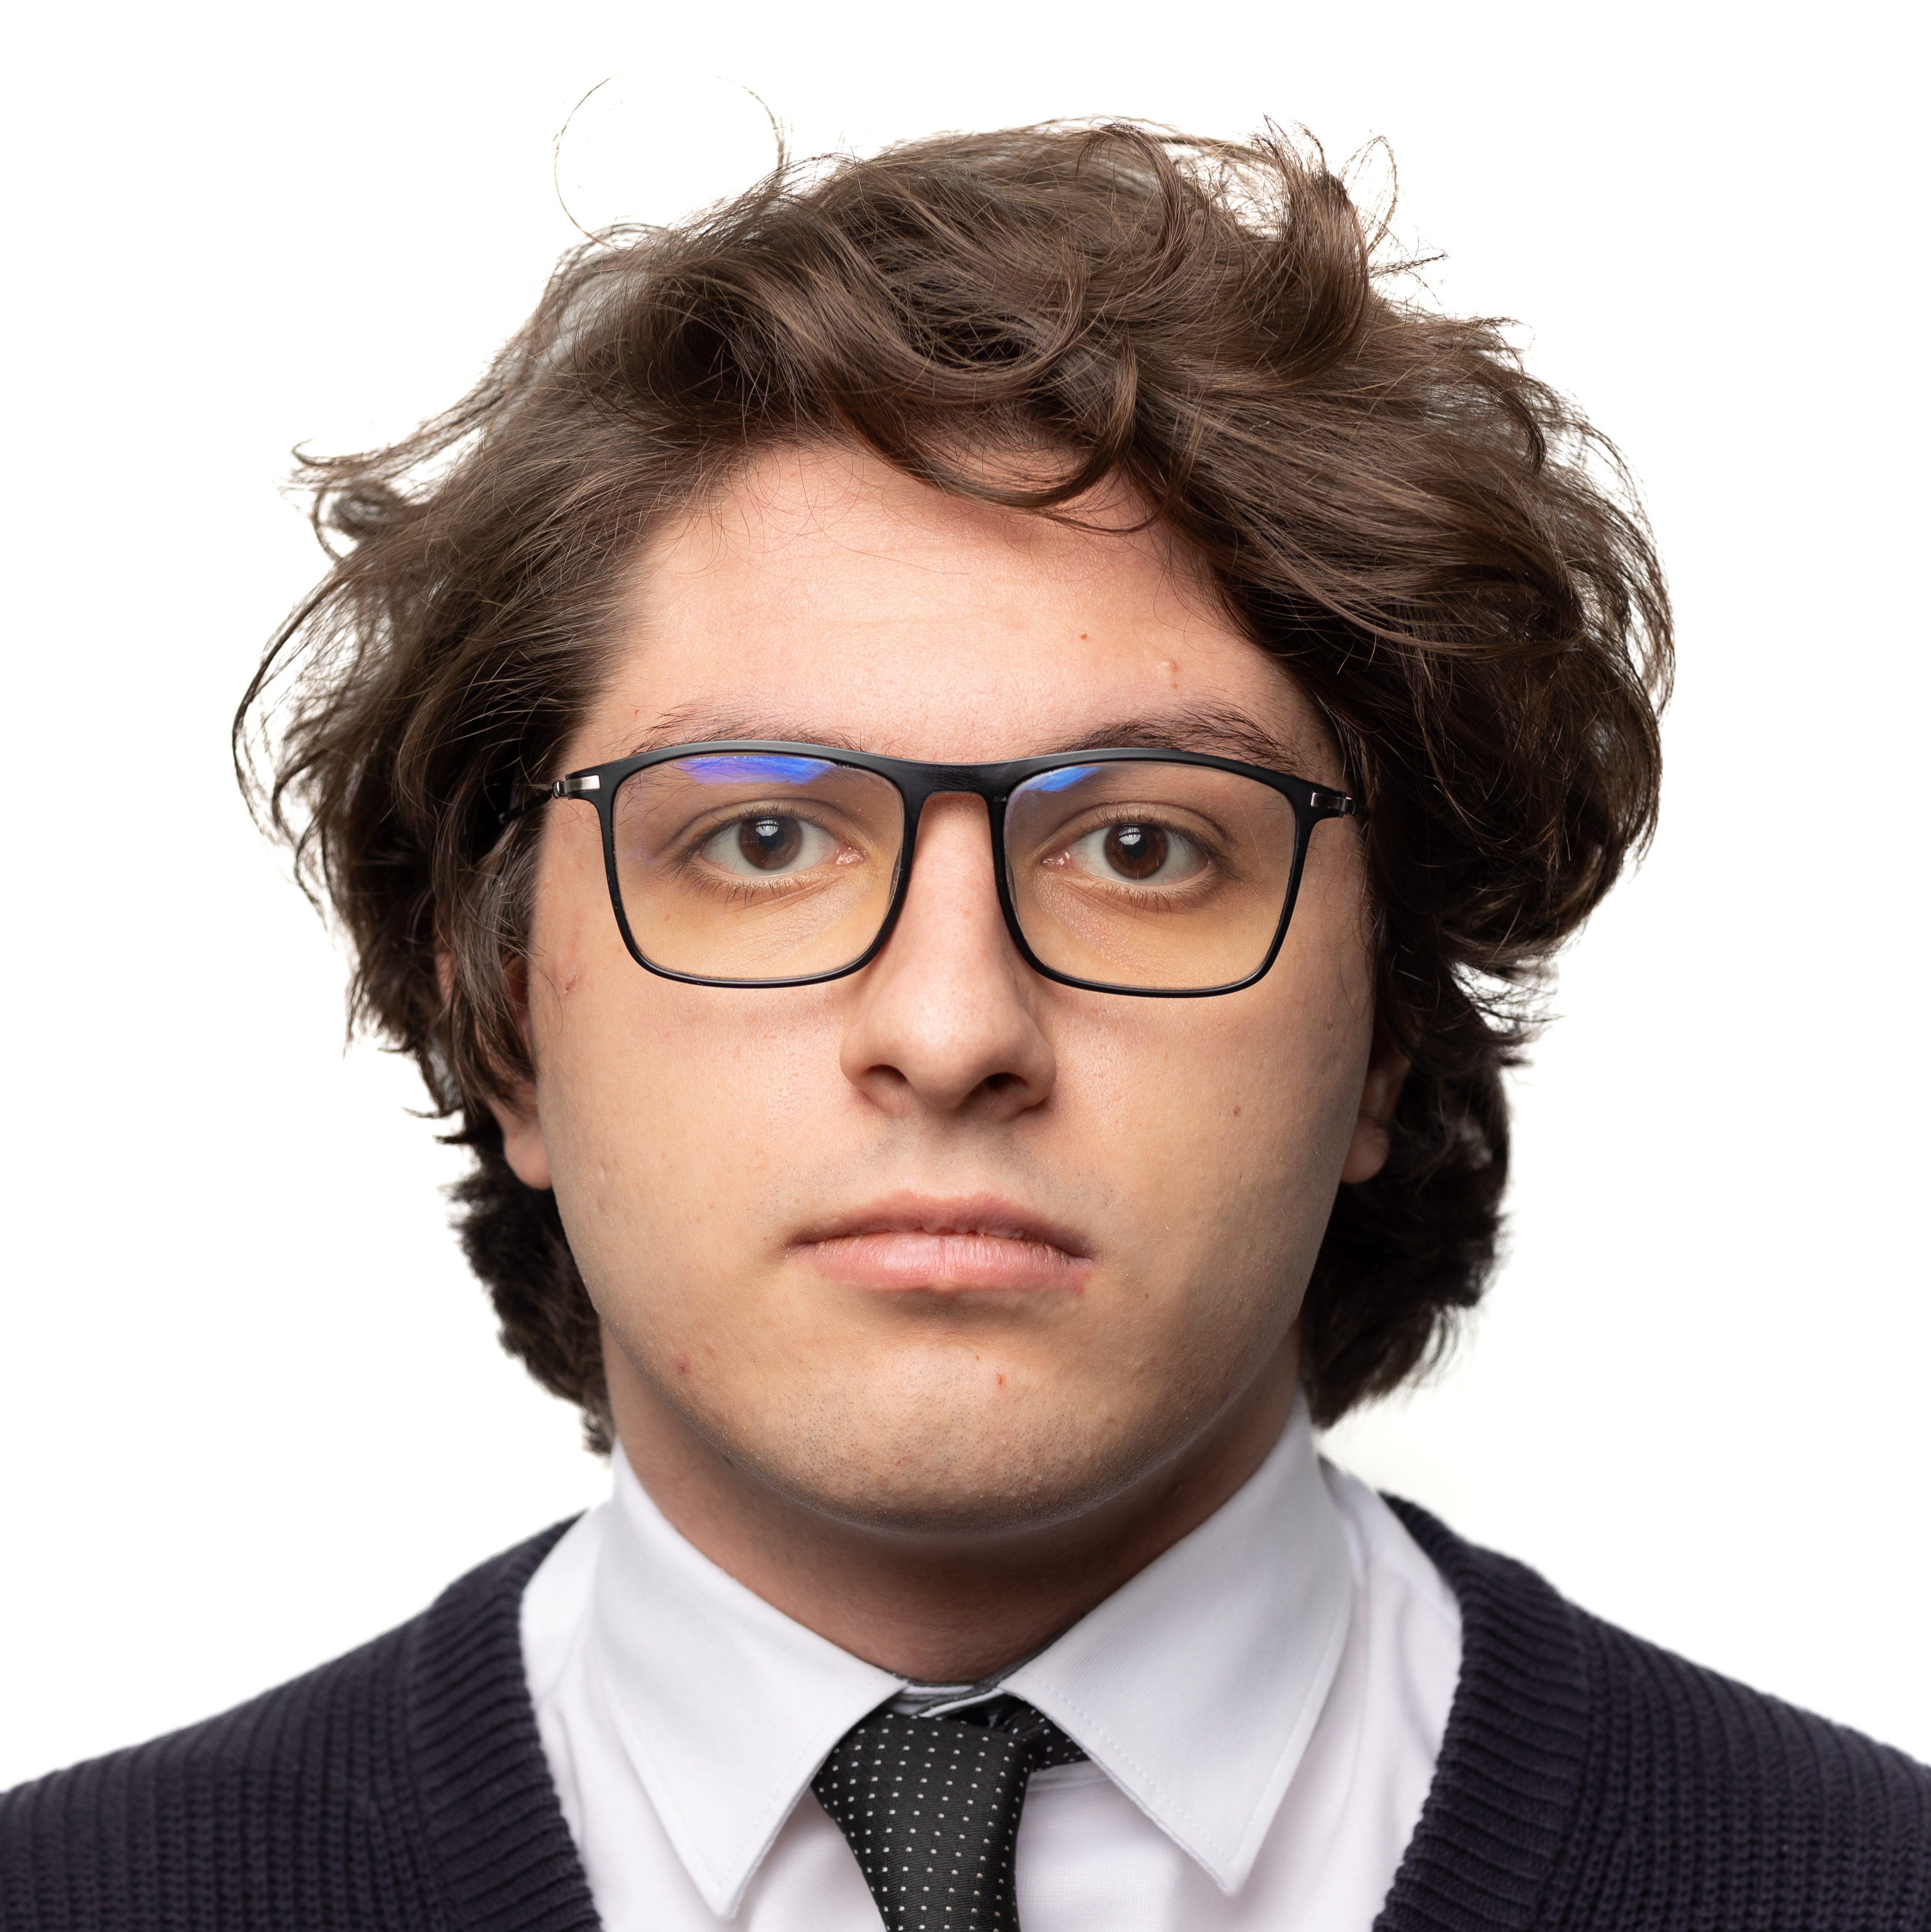
\includegraphics[width=3cm]{STOP2008-rect.jpg}
\end{textblock}

\begin{center}
    \small{
    +40-722-594-770 | \href{mailto:vladtomici@gmail.com}{vladtomici@gmail.com} |
    \href{https://vladtomici14.github.io/}{https://vladtomici14.github.io/}
    }
\end{center}
\vspace{-6mm}

\begin{center}
    \small{
    \socialicon{\faLinkedin} \href{https://www.linkedin.com/in/vlad-tomici/}{Profil de LinkedIn} |
    \socialicon{\faGithub} \href{https://github.com/VladTomici14}{Profil de GitHub} |
    }
\end{center}
\vspace{-6mm}
\begin{center}
    \small{Timișoara, România}
\end{center}
\end{minipage}

\vspace{4mm}

\section{\textbf{Despre mine}}
\vspace{1mm}
\small{
\textit{Student în anul III} @ \textbf{Facultatea de Automatică și Calculatoare}, \textit{Departamentul de Calculatoare și Tehnologia Informației}. \newline

\textit{Vicepreședinte Interne} @ \textbf{Liga AC}. \newline


% Ocazional, lucrez ca freelancer pe proiecte de Computer Vision, Python și Machine Learning. \newline

Tânăr programator devotat, cu bune abilități de comunicare și management al echipei. Vorbitor de limba engleză, cu certificare Cambridge English C1.\newline

Experiență în participarea la hackathoane locale și concursuri de programare din România. Cunoștințe de dezvoltare a proiectelor de Computer Vision și Machine Learning în Python, rezolvarea problemelor algoritmice în C/C++, crearea de aplicații simple Java, Kotlin și Swift și aplicații web Angular / .NET. Capabil să proiectez, să construiesc și să programez roboți folosind microcontrolere. Nivel mediu de cunoștințe în electronică.\newline

Pasionat de domeniul tehnologiei, din 2016.

% Fost formator în \textbf{Clubul de Dezbateri Solaris}, parte a \textit{ACDV} (Asociația Cluburilor de Dezbateri din Vest).\newline

% Mentor în comunitatea locală \textbf{CoderDojo}.
}
\vspace{-2mm}



\section{\textbf{Experiență profesională}}
\vspace{-0.4mm}
  \resumeSubHeadingListStart
        \resumeSubheading
        {{AUMOVIO [\href{https://www.aumovio.com/en.html}{\faIcon{globe}}]}}{Timișoara, România}
          {Internship AI Developer}{Iun 2026 - Prezent}

        \resumeItemListStart
            \item Dezvoltarea de aplicații și agenți AI care automatizează fluxurile de lucru interne din inginerie.
            \item Construirea de soluții de clasificare, ranking și consiliere care sprijină developerii și inginerii în activitatea de zi cu zi.
            \item Lucrul cu LLM-uri self-hosted, pipeline-uri Jenkins și codebase-uri existente, pentru integrarea instrumentelor AI în procesele de dezvoltare.
        \resumeItemListEnd

      \resumeOrg
        {{Liga AC [\href{https://ligaac.ro}{\faIcon{globe}}]}}{Timișoara, România}
        \resumeRole{Vicepreședinte Interne}{Sep 2026 - Prezent}
        
        \resumeItemListStart
            \item Parteneriate cu industria: Conectez comunitatea noastră de studenți cu industria tech, purtând discuții cu companii private pentru a obține sprijinul care face posibile proiectele noastre.
            \item Coordonarea echipelor: Coordonez echipele de voluntari pentru ca evenimentele să se desfășoare fără probleme, de la planificare până la execuție.
            \item Evenimente educaționale: Îi sprijin pe colegii mei în crearea unor evenimente educaționale valoroase pentru studenți.
        \resumeItemListEnd

        \resumeRole{Coordonator Departament Tehnic}{Sep 2025 - Sep 2026}

        \resumeItemListStart
            \item Infrastructură \& DevOps: Am administrat infrastructura Linux pe VPS, reverse proxy-uri Nginx și baze de date MariaDB pentru platforme cu trafic ridicat.
            \item Automatizare \& Scalabilitate: Am construit pipeline-uri CI/CD în GitLab și medii containerizate Docker pentru aplicații .NET, Angular și aplicații Python de procesare a datelor.
            \item Leadership tehnic: Am coordonat o echipă de 5 Technical Project Manageri, asigurând respectarea standardelor de cod și integrarea sistemelor prin code review-uri constante și întâlniri 1-la-1.
        \resumeItemListEnd

      \resumeSubheading
          {{Freelancer}}{Remote}
          {Dezvoltator Machine Learning și Python}{Mar 2022 - Mai 2026}
          \resumeItemListStart
            \item Dezvoltare ML end-to-end: Am proiectat și implementat soluții ML complete, acoperind întregul flux de lucru, de la procesarea datelor brute până la integrarea modelelor în aplicații funcționale.
            \item Computer Vision \& Deep Learning: Am aplicat tehnici avansate de procesare a imaginilor și arhitecturi de Deep Learning (Transfer Learning) pentru rezolvarea unor probleme complexe de detecție și clasificare în medii dinamice.
            \item Pipeline-uri de date automatizate: Am dezvoltat scripturi Python de optimizare pentru extragerea, curățarea și transformarea seturilor de date, asigurând calitatea datelor de intrare pentru antrenarea modelelor.
            \item Integrare cross-platform: Am colaborat la integrarea modulelor AI în diverse ecosisteme software (mobile și desktop), adaptând algoritmii în funcție de cerințele de performanță ale clienților.
          \resumeItemListEnd

      \resumeSubheading
          {{Data Annotation}}{Remote}
          {Data Annotator}{Iul 2024 - Dec 2024}
          \resumeItemListStart
            \item Generarea de prompturi și evaluarea răspunsurilor oferite de chatboți pe teme legate de programare.
          \resumeItemListEnd

      \resumeSubheading
          {{Endava [\href{https://drive.google.com/file/d/1LKCoWz4KD9qf3SZpea_x3N-8CAprefYC/view?usp=sharing}{\faIcon{globe}}]}}{Timișoara, România}
          {Student Intern}{Iul 2022}
          \resumeItemListStart
            \item Am finalizat un program intensiv de internship de o săptămână, dobândind cunoștințe teoretice și practice avansate și contribuind la rezultatele proiectului.
          \resumeItemListEnd

  \resumeSubHeadingListEnd
\vspace{-6mm}

\section{\textbf{Studii}}
\vspace{-0.4mm}
\resumeSubHeadingListStart

\resumeSubheading
{Facultatea de Automatică și Calculatoare}{Timișoara, România}{Licență în Ingineria Calculatoarelor, Departamentul de Calculatoare și Tehnologia Informației}{Oct 2024 - Prezent}

\resumeSubheading
{Liceul Teoretic "Grigore Moisil"}{Timișoara, România}{Studii liceale}{Sep 2020 - Iul 2024}

\resumeSubHeadingListEnd
\vspace{-6mm}


\section{\textbf{Informații suplimentare}}
% \vspace{-0.4mm}
\small{
\textbf{Limbi străine:}
\resumeItemListStart
    \item Română \textit{(Limba maternă)}
    \item Engleză \textit{(Nivel profesional)}
    \item Germană \textit{(Nivel elementar)}
\resumeItemListEnd
\vspace{2mm}


\textbf{Interese:} lectură, fotbal, drumeții
}


\section{\textbf{Competențe}}
\vspace{-0.4mm}
 \resumeHeadingSkillStart
   \resumeSubItem{Competențe personale: }
    {comunicare, rezolvarea problemelor complexe, lucru în echipă, inteligență emoțională, curiozitate}
  \resumeSubItem{Limbaje de programare: }
    {Python (avansat), C/C++ (algoritmi \& embedded), C\#, Java}
  \resumeSubItem{AI \& Machine Learning: }
    {TensorFlow, Keras, PyTorch, OpenCV, Scikit-learn, procesare de imagini}
  \resumeSubItem{Data Science \& Machine Learning: }
    {TensorFlow, Keras, PyTorch, OpenCV, Matplotlib, Jupyter Notebook}
  \resumeSubItem{Web \& Backend:}
    {Angular, .NET, MariaDB/SQL, Nginx}
  \resumeSubItem{Embedded: }
    {Raspberry Pi, Arduino, microcontrolere}
  \resumeSubItem{Alte tehnologii: }
    {Linux, Git}
 \resumeHeadingSkillEnd


\section{\textbf{Licențe \& Certificări}}
\vspace{-0.2mm}
\resumeSubHeadingListStart

\resumePOR{}{\href{https://drive.google.com/file/d/1WMnR9FlJT_pPSB15GxZpJTv662y901Cq/view?usp=sharing}{
\textbf{Curs de Fundamente ale Calculului și Comunicațiilor Cuantice - (RoNaQCI)}
}}{Dec 2024}

\resumePOR{}{\href{https://drive.google.com/file/d/1SCBSCP2LY4lAmFC1qx0hxTLmfbSR4jCO/view?usp=sharing}{
\textbf{Cambridge English: Advanced (CAE)}
}}{Dec 2023}

\resumePOR{}{\href{https://drive.google.com/file/d/1R3IxChVuiy-t4H5uhFsGPcKmu4DS51Wh/view?usp=sharing}{
\textbf{IC3 Certification - Global Standard 5)}
}}{Ian 2023}

\resumePOR{}{\href{https://drive.google.com/file/d/1SIY_7KhyOPoYnHBO6ikptXtp6GIHQ3-v/view?usp=sharing}{
\textbf{Cambridge English: Preliminary (PET))}
}}{Mai 2021}

% \resumePOR{}{\href{https://drive.google.com/file/d/1S9i8Lo0IzSALQ03V_4R9xibqxaHYoIQH/view?usp=sharing}{
% \textbf{Cambridge English: Key (KET))}
% }}{Mai 2018}

% \resumePOR{}{\href{https://drive.google.com/file/d/1S9SIVcP5MvXS2PAEMleNpXJqqIVLhNhJ/view?usp=sharing}{
% \textbf{Cambridge English: Flyers (YLE Flyers)}
% }}{Mai 2017}

% \resumePOR{}{\href{https://drive.google.com/file/d/1SGIGNVZuOUZEpklmOd8kzs3Kraowclcx/view?usp=sharing}{
% \textbf{Cambridge English: Movers (YLE Movers))}
% }}{Mai 2016}

% \resumePOR{}{\href{https://drive.google.com/file/d/1SDDmP1nszUsatExw6in075_eUzrp4SDo/view?usp=sharing}{
% \textbf{Cambridge English: Starters (YLE Starters)}
% }}{Mai 2015}

\resumeSubHeadingListEnd
\vspace{-6mm}

% \section{\textbf{Proiecte}}
% \vspace{-0.4mm}
% \resumeSubHeadingListStart

% \resumeProject
%   {Propagarea Undelor}
%   {Tehnologii utilizate: Python, NumPy, Matplotlib, Jupyter Notebook}
%   {Dec 2024 - Ian 2025}
%   {{}[\href{https://github.com/VladTomici14/wave-propagation-visualisation}{\textcolor{darkblue}{\faGithub}}]}
% \resumeItemListStart
%   \item Simulare numerică pentru a vizualiza propagarea undelor în 2+1 dimensiuni.
%   \item Pe baza unei formule de undă date, proiectul creează o vizualizare 3D interactivă a evoluției undei.
% \resumeItemListEnd

% \resumeProject
%   {DOCScan: aplicație iOS pentru scanarea documentelor, extragerea textului și gestionarea documentelor digitale}
%   {Tehnologii utilizate: Swift, SwiftUI, Python, Firebase}
%   {Mar 2024 - Iun 2024}
%   {{}[\href{https://github.com/VladTomici14/DOCScan}{\textcolor{darkblue}{\faGithub}}]}
% \resumeItemListStart
%   \item Dezvoltat folosind SwiftUI și Firebase pentru autentificare și stocare în cloud.
%   \item Utilizează computer vision pentru a detecta documentele și a îmbunătăți imaginile scanate.
%   \item Am implementat un NLP pentru extragerea și procesarea precisă a textului.
%   \item Dezvoltat drept atestat de absolvire a liceului.
% \resumeItemListEnd

% \resumeProject
%   {Recunoașterea emoțiilor}
%   {Tehnologii utilizate: Python, TensorFlow, OpenCV, NumPy, Matplotlib}
%   {Apr 2022}
%   {{}[\href{https://github.com/VladTomici14/Emotion-recognition-through-transfer-learning}{\textcolor{darkblue}{\faGithub}}]}
% \resumeItemListStart
%   \item Am construit un model de recunoaștere a emoțiilor folosind arhitectura VGG16.
%   \item Am aplicat transfer learning și un CNN pentru clasificarea expresiilor faciale.
%   \item Detecția emoțiilor funcționează în timp real, dar și pe imagini, cu suport pentru cameră web.
% \resumeItemListEnd

% \resumeProject
%   {eBon: Bonuri digitale pentru o experiență de cumpărături modernă și ecologică}
%   {Tehnologii utilizate: programare pe Raspberry Pi, Flutter, Python, Firebase}
%   {Dec 2021}
%   {{}[\href{https://github.com/mihai-albu03/eBon}{\textcolor{darkblue}{\faGithub}}]}
% \resumeItemListStart
%   \item Am construit componenta hardware bazată pe Raspberry Pi.
%   \item Am contribuit la dezvoltarea aplicației Flutter a proiectului.
%   \item Am integrat atât aplicația, cât și componenta hardware cu un backend Firebase.
%   \item Dezvoltat în cadrul hackathonului internațional UniHack 2021, împreună cu 2 colegi de liceu.
% \resumeItemListEnd

% \resumeProject
%   {Rusty: un simplu robot cu Raspberry Pi}
%   {Tehnologii utilizate: Python, procesare de imagini, electronică, modelare și printare 3D}
%   {Oct 2018 - Mai 2021}
%   {{}[\href{https://github.com/VladTomici14/Rusty6}{\textcolor{darkblue}{\faGithub}}]}
% \resumeItemListStart
%   \item Proiectat pentru operațiuni în zone periculoase sau greu accesibile.
%   \item Echipat cu senzori de temperatură \& umiditate, ultrasonici și de gaz. Alimentat de un panou solar, are o cameră care ajută la procesarea imaginilor pentru detecția persoanelor.
% \resumeItemListEnd

% \resumeSubHeadingListEnd


% \section{\textbf{Premii \& Distincții}}
% \vspace{-0.4mm}
% \resumeSubHeadingListStart

% \resumeProject
%   {Câștigător al categoriei "Technology 4 Health (High School)"}
%   {HackTM 2023}
%   {Mai 2023}
%   {{}[\href{https://github.com/VladTomici14/NeuroVault}{\textcolor{darkblue}{\faIcon{globe}}}]}
% \resumeItemListStart
%   \item Am dezvoltat o aplicație web care ajută la integrarea în societate a persoanelor cu autism, printr-o comunicare mai eficientă între pacienți, specialiști și apropiații pacienților.
%   \item NeuroVault permite crearea unui profil în care specialiștii pot nota comportamentele pacientului și consecințele acestora, astfel încât interacțiunile viitoare să fie mai eficiente.
%   \item Am dezvoltat partea de back-end a aplicației și baza de date, folosind JavaScript și PHP.
% \resumeItemListEnd

% \resumeProject
%   {Intelligent Electricity Generation - Locul 2}
%   {Facultatea de Electrotehnică și Electroenergetică}
%   {Mai 2023}
%   {{}[\href{https://drive.google.com/file/d/1lGNVWn66y1pjQws85YHQjKOu8DPgJblN/view?usp=sharing}{\textcolor{darkblue}{\faIcon{globe}}}]}
% \resumeItemListStart
%   \item Am participat cu robotul de competiție al echipei WizzTech din sezonul 2022-2023.
%   \item Premiu câștigat ca membru al echipei de robotică WizzTech.
% \resumeItemListEnd

% \resumeProject
%   {AI Development, categoria Advanced - Locul 3}
%   {iTEC 2022}
%   {Mai 2022}
%   {{}[\href{https://github.com/VladTomici14/iTEC2022}{\textcolor{darkblue}{\faIcon{globe}}}]}
% \resumeItemListStart
%   \item Am dezvoltat o rețea neuronală pentru clasificarea formelor și culorilor.
%   \item Am construit un generator aleatoriu de seturi de date cu figuri geometrice și am implementat un model bazat pe DenseNet, cu o acuratețe de ~98\% la antrenare.
%   \item Am folosit Python, TensorFlow, Keras și OpenCV pentru antrenare și clasificare.
% \resumeItemListEnd

% \resumeProject
%   {AI Development - Mențiune}
%   {iTEC 2021}
%   {Mai 2021}
%   {{}[\href{https://drive.google.com/file/d/1Rz9LomgwTDH7vVcHF6-qTt6ez0EfQ5Sy/view?usp=sharing}{\textcolor{darkblue}{\faIcon{globe}}}]}
% \resumeItemListStart
%   \item Am dezvoltat aplicația VerificAI în Microsoft Power Apps, pentru automatizarea gestionării stocurilor din magazine.
% \resumeItemListEnd

% \resumeProject
%   {Software utilitar și jocuri - Locul 1}
%   {Concursul Național de Software "Grigore Moisil"}
%   {Mai 2019}
%   {{}[\href{https://drive.google.com/file/d/1NNBqmOeLKyS263kS18LnMv4gZyOTtFkk/view?usp=sharing}{\textcolor{darkblue}{\faIcon{globe}}}]}
% \resumeItemListStart
%   \item Am dezvoltat un robot cu Raspberry Pi controlat de la distanță, echipat cu o Pi Camera care transmite imagini în timp real.
% \resumeItemListEnd

% \resumeProject
%   {Categoria Freestyle - Locul 3}
%   {RoboTEC 2019}
%   {Apr 2019}
%   {{}[\href{https://drive.google.com/file/d/1VEAFCbDciYrWjKh9K-pOFRntG6ccpXGp/view?usp=sharing}{\textcolor{darkblue}{\faIcon{globe}}}]}
% \resumeItemListStart
%   \item Am participat cu un robot construit pe platforma Raspberry Pi, folosind câțiva senzori de bază și 4 motoare.
% \resumeItemListEnd

% \resumeSubHeadingListEnd



\section{\textbf{Experiență de voluntariat}}
\vspace{-0.4mm}
\resumeSubHeadingListStart

\resumeOrg
  {{Echipa de robotică WizzTech [\href{https://github.com/WizzTech-RO048}{\faIcon{globe}}]}}{Timișoara, România}
  \resumeRole{Mentor}{Aug 2024 - Mar 2026}
\resumeItemListStart
  \item Asigur comunicarea cu sponsorii și partenerii.
  \item Am atras peste 6000\texteuro{} din sponsorizări pentru bugetul echipei.
  \item Mentorat în programare Java, dezvoltarea roboților și modelare 3D.
  \item Asigur un mediu prietenos și colaborativ, în care fiecare elev de liceu se poate bucura de robotică într-un cadru competitiv.
\resumeItemListEnd

  \resumeRole{Lider de echipă}{Sep 2022 - Mar 2024}
\resumeItemListStart
  \item Am condus o echipă de peste 15 elevi de liceu, timp de 3 sezoane consecutive, în FIRST Tech Challenge, una dintre cele mai mari competiții internaționale de robotică pentru liceeni.
  \item Am organizat \textbf{WizzTech League Meet}: o competiție locală de robotică cu peste 80 de participanți. M-am ocupat de logistică, comunicare și arbitraj.
  \item Am co-organizat \textbf{Academia WizzTech}: o serie de workshop-uri și prezentări pentru liceenii interesați de robotică.
  \item Am atras peste 3000\texteuro{} din sponsorizări pentru bugetul echipei.
  \item Am asigurat comunicarea cu sponsorii și partenerii.
  \item Toate acestea în timp ce eram programatorul principal al echipei.
\resumeItemListEnd

\resumeProject
  {Trainer \& Organizator}
  {Clubul de Dezbateri Solaris}
  {Sep 2021 - Feb 2024}
  {{}[\href{https://acdv.ro/cluburi/}{\textcolor{darkblue}{\faIcon{globe}}}]}
\resumeItemListStart
  \item Am pregătit și îndrumat peste 50 de elevi de liceu, timp de 2,5 ani consecutivi, în formatul de dezbatere World Schools (argumentare, strategie și documentare), prin sesiuni de antrenament, workshop-uri și pregătire pentru competiții.
  \item Am co-organizat \textbf{Moisil Summer Open 2023}: o competiție locală de dezbateri cu peste 120 de participanți. M-am ocupat de logistică și finanțare.
\resumeItemListEnd

\resumeSubHeadingListEnd
\vspace{-6mm}

\vspace{-4mm}

\end{document}
